\documentclass[12pt]{article}
\usepackage[utf8]{inputenc}
\usepackage[T1]{fontenc}
\usepackage{graphicx} % Required for inserting 
\graphicspath{{../Figures/}}
\usepackage{figure_dirs}
\usepackage[hidelinks, colorlinks=true, linkcolor=blue, citecolor=cyan]{hyperref}
\usepackage[
    a4paper,
    margin=1in
    ]{geometry}
\usepackage{mathtools}
\usepackage{amssymb, amsthm}
\usepackage{math}
\usepackage{setspace}
\usepackage{booktabs}
\usepackage{makecell}
\usepackage{titlesec}
% \usepackage{natbib}
\titleformat*{\section}{\Large\bf}
\titleformat*{\subsection}{\large\bf}
\titleformat*{\subsubsection}{\normalsize\bf}
\usepackage{chngcntr}
\usepackage{lipsum}
\usepackage[labelfont=bf, labelsep=period]{caption}
\usepackage[capposition=top]{floatrow}
\usepackage{enumitem}
\usepackage{mathrsfs}
% \usepackage{fourier}
% \usepackage{newtx}
\newtheorem{thm}{Theorem}
\newtheorem*{thm*}{Theorem}
\newtheorem{defn}{Definition}
\newtheorem*{defn*}{Definition}
\newtheorem{axiom}{Axiom}
\newtheorem*{axiom*}{Axiom}
\renewcommand{\theaxiom}{B\arabic{axiom}}
\newtheorem{ax}{Axiom}
\newtheorem*{ax*}{Axiom}
\renewcommand{\theax}{A\arabic{ax}}
\newtheorem{lemma}{Lemma}
\newtheorem{prop}{Proposition}
\newtheorem*{prop*}{Proposition}
\newtheorem{crl}{Corollary}
\newtheorem{remark}{Remark}[section]

\newcommand{\Rfix}{\mathsf{R}}
\newcommand{\Rfree}{\Re}
\renewcommand{\vs}{\varsigma}
\renewcommand{\Rc}{\Rs}
\renewcommand{\Gc}{\Gs}

\newcommand{\pref}{\succcurlyeq}
\newcommand{\sm}{\setminus}
\newcommand{\prefs}{R}
\newcommand{\succs}{P}
\newcommand{\sims}{I}
\newcommand{\rev}[1]{#1^{-}}

\newcommand{\pf}{\noindent\textbf{Proof: }}

\newcommand{\cd}{Draft 2} % Choose the version of the paper to render

\newcommand{\pdd}[3]{\frac{\partial^2 #1}{\partial {#2}^2}\Bigg|_{#3}}
\newcommand{\pcd}[4]{\frac{\partial^2 #1}{\partial {#2} \partial {#3}}\Bigg|_{#4}}

% \newcommand{\pd2}[3]{\frac{\partial^2 #1}{\partial {#2}^2}\Big|_{#3}}

% \usepackage[authordate, backend=biber, maxcitenames=2, natbib=true]{biblatex-chicago}
% \addbibresource{correlated_shocks_equity_premium.bib}
\usepackage{natbib}
\usepackage[hang, flushmargin]{footmisc}

\usepackage{caption}
\usepackage{subcaption}

\makeatletter

% make numeric styles use name format
\patchcmd{\NAT@test}{\else \NAT@nm}{\else \NAT@nmfmt{\NAT@nm}}{}{}

% define \citepos just like \citet
\DeclareRobustCommand\citepos
  {\begingroup
   \let\NAT@nmfmt\NAT@posfmt% ...except with a different name format
   \NAT@swafalse\let\NAT@ctype\z@\NAT@partrue
   \@ifstar{\NAT@fulltrue\NAT@citetp}{\NAT@fullfalse\NAT@citetp}}

\let\NAT@orig@nmfmt\NAT@nmfmt
\def\NAT@posfmt#1{\NAT@orig@nmfmt{#1's}}

\makeatother

% \renewcommand{\mkbibnamefamily}[1]{\textsc{#1}}


% \makeatletter
% \@addtoreset{prop}{section}
% \makeatother

\title{Portfolio choice with correlated income growth and equity return shocks
\let\thefootnote\relax\footnotetext{I thank Chris Carroll, Lalit Contractor, and Alan Lujan for their comments and suggestions. Any remaining errors are my own.}
}
\author{Siddarth Venkatesh\thanks{Ashoka University, email: \texttt{siddarth.venkatesh\_tf@ashoka.edu.in}\\\hspace*{1.8em}The \href{https://github.com/econ-ark/HARK/pull/1412}{multivariate lognormal} discretization code I use to solve this model is available in the \href{https://github.com/econ-ark/HARK}{HARK} toolkit.}}
\date{This Version: March 05, 2025 % Draft 2 date}

% \setlength{\parindent}{0pt}
% \setlength{\parskip}{1em}

\begin{document}

\maketitle
\begin{abstract}
    \lipsum[50]
\end{abstract}

\linespread{1.15}

%\section{Introduction}

The standard buffer stock model \citep{Deaton1991, Carroll1992} predicts that consumers engage in precautionary saving either because of borrowing constraints or the possibility of unemployment. Despite this, under a canonical formulation with independent shocks to income and returns on equity, the model counterintuitively predicts that poor consumers should invest their entire savings in equity, while wealthy consumers should save in the safe asset.\footnote{The one exception is that with zero income events, arbitrarily poor consumers invest the same fraction of their savings in equity as the arbitrarily wealthy.} The predictions of lifetime portfolio optimization models by \citet{Merton1969, Samuelson1969} suggest that the major component in the willingness to invest in the risky asset arises from a regular income stream \citep{Heaton1997}. 

\citet{Kimball1991} showed that consumers may display a temperance motive to moderate exposure to other risks when faced with income uncertainty, even if these risks are statistically independent. \citet{Koo1999} shows that an increase in the volatility of permanent income growth shocks significantly amplifies the temperance effect, though transitory income shocks have negligible influence. This does not change a key prediction of the model, however, that the poor should invest all their savings in equity, and the portfolio share of equity declines with wealth. Furthermore, given the equity premium and the volatility of returns on stock observed in the data \citep{Mehra1985}, the baseline model suggests that even the wealthy should invest all their savings in stocks.

One explanation for the modest portfolio share of equity observed in the data is that future consumption is positively correlated with returns on equity. \citet{Constantinides2002} use an overlapping generations (OLG) model to explore this idea. In their model, there are three generations of individuals: the young, middle-aged, and old/retired. Retired individuals receive a labor income of zero, which means that the future consumption of the middle-aged is highly correlated with the returns on equity. On the other hand, the middle-aged face uncertain wage income, implying that the future consumption of the young depends on more than just the returns on equity, lowering their correlation. Their argument is that a positive correlation implies that the realization of low marginal utility of consumption coincides with high returns, and vice versa. Thus, the low portfolio share of equity is a consequence of the inability of the young to participate in the stock market due to borrowing constraints. This paper departs from their modeling assumptions by retaining income uncertainty and introducing correlations between permanent income growth shocks and equity returns to correlate future consumption and equity returns. A positive correlation between these shocks reduces the potential of equity risk to serve as a hedge against fluctuations in future consumption due to permanent income growth risk.

This paper primarily focuses on an infinitely-lived agent\footnote{The setup is well-suited to life-cycle modeling, but the insights derived in this paper are from the predictions of the infinite-horizon model.} who consumes a single good and maximizes the discounted sum of utility from consumption. The agent faces three risks: shocks to the return on equity, permanent income growth, and transitory income. The model can accommodate pairwise correlations between all three shocks, though the focus of this paper will be on the case where permanent income shocks and equity returns are correlated, while transitory income shocks are independent of both. The agent decides their consumption (therefore, saving) and the portfolio share of equity in every period. The flexibility of the model in terms of the distribution of the shocks allows us to establish that a correlation between transitory income shocks and equity returns has a negligible effect on the portfolio share of equity for all agents but those with near-zero savings.

There is ample justification in the literature to model permanent income growth as correlated with equity returns while modeling transitory income shocks as independent of the two. \citet{Campbell1996} shows that there is a high correlation between the present value of human capital and market returns, despite finding that the contemporaneous correlation between wage income and stock returns is low. However, the source of this covariance in his model is due to a common time-varying discount factor applied to both calculations. \citet{Baxter1997} also find that the correlation between the returns to human capital and physical capital are high, even as labor and capital income growth rates may not exhibit a high correlation. With independent shocks across time, permanent income growth proportionally affects the expected present discounted value of human capital, while the independent transitory shock allows for the low correlation in actual labor income growth and returns on equity.

There have been papers that have studied correlations between labor income growth and equity returns previously in a life-cycle setting. \citet{Bodie1992} modelled the labor supply decision as endogenous, and made after the current return to equity has been determined. They show that agents vary their labor supply ex-post to cushion themselves against greater risks taken in their investment decisions. Subsequent papers study this relationship with an exogenous income process and a positive relationship between income growth and equity returns. \citet{Benzoni2007} explore a model with cointegrated labor income and stock market returns in a continuous-time setting. \citet{Bagliano2014} on the other hand study a discrete-time model with a permanent income shock that has both an aggregate and an idiosyncratic component, and two risky assets. The closest paper to mine is by \citet{Viceira2001}, whose model is based on a similar buffer-stock setting with correlations between permanent income growth and risky asset returns. The difference here is that I focus on the problem of the infinitely-lived agent, whose income is subject to both transitory and permanent income shocks, and who may face an artificial borrowing constraint instead of possible spells of unemployment that otherwise serves as the motive for precautionary saving. My focus, thus, is on portfolio choice across the wealth distribution and around the target wealth, as opposed to over the life-cycle.

The imposition of the artificial borrowing constraint serves multiple purposes. First, in a model trying to understand the long-term equity holdings of consumers, it abstracts away from short-selling behavior. Then, it avoids any discontinuities in the problem at the point where savings are zero. Most lucratively, however, the consumer who faces artificial borrowing constraints tends to save very little at their target wealth and therefore invests none of their savings in equity, lending support to the well-studied argument that borrowing constraints among the young, for instance, can cause reduced or non-participation in the stock market \citep{Constantinides2002, Haliassos2002, Kogan2007, Jang2015, Harenberg2018}. I also artificially restrict the portfolio share of equity to between 0 and 1, which implies that consumers cannot hold debt-financed equity positions. \citet{Davis2006} argue that borrowing costs can be a major deterrent against investing in equity using loans, and it is beyond the scope of this paper to examine the differences in rates of return and mechanisms available for consumers to borrow versus save.

The findings of this paper can be divided into three major strands. First, a positive correlation between permanent income growth shocks and returns on equity does have a negative effect on the portfolio share of equity of an agent with a moderate level of risk aversion ($\rho = 4$). This effect is primarily observed among the poor who save very little, and gradually disappears for extremely wealthy agents. As wealth tends to infinity, the portfolio share of equity tends to the value in the \citet{Merton1969,Samuelson1969} case, irrespective of the correlation between income and equity return shocks. Second, for moderate to high levels of correlation between the permanent income growth and equity return shocks, the optimal portfolio share of equity is actually increasing in wealth, unlike the model with uncorrelated shocks. Third, with the artificial borrowing constraint, agents do not invest in equity or invest extremely small proportions of their savings in it around the target level of wealth, while the threat of unemployment better explains the portfolio share of equity around target levels of wealth conditional on participation in the stock market. Though the model generates insightful predictions for an equity premium set at 3 percent with the standard deviation of the logged shock to the return set at 15 percent, calibrating the model to parameters implied by data on U.S. equity returns as reported in \citet{Mehra2006} necessitates an elevated risk aversion parameter of around 7 to generate modest portfolio shares of equity around target wealth. 

The covariance of permanent income growth and returns on equity is, of course, one among multiple theories posited to resolve the equity premium puzzle. A section of the literature argues that habit-formation makes consumers more averse to the volatility in consumption across time-periods induced by the risk on equity return \citep{Constantinides1990, Abel1990, Detemple1991, Campbell1999, Otrok2002}. Another strand of the literature focuses on the low participation rates in the stock market despite the large equity premium and uses market frictions like fixed participation costs to explain increasing participation with age and wealth \citep{Cocco2005, Gomes2005, Alan2006, Khorunzhina2013, Fagereng2017}. Modest portfolio shares of equity are also explained by heterogeneous and pessimistic beliefs about the returns on stocks. The evidence suggests that beliefs about the volatility of returns on equity are exaggerated, and portfolio decisions are correlated with the reported beliefs about the stock market \citep{Dominitz2007, Hurd2011, Amromin2014, Ameriks2020, Mateo2024}. Yet another explanation revolves around departures from expected utility preferences \citep{Haliassos1995,Haliassos2001, Routledge2010, Schreindorfer2020}.\footnote{See \citet{Barucci2003} for a detailed exploration of the assumptions imposed under the standard rational paradigm and the puzzles that stem from relaxing them.} Section \ref{reconciliation} discusses how some of these explanations may tie in with the model in this paper to favorably revise the predictions of the model without requiring a large coefficient of relative risk aversion.

The paper is structured as follows. Section \ref{model} sets up the model and discusses the solution method used. Section \ref{results} examines predictions from the model with the artificial no-borrowing constraint. Section \ref{zero_inc} relaxes the borrowing constraint and introduces the possibility of unemployment in the income process. Section \ref{discussion} provides a few comments and concludes.

\section{Model}

\subsection{The basic problem}

I start by examining the basic consumption-saving problem. The individual maximizes their discounted lifetime utility from the consumption stream $\bc{C_{t}}_{t=0}^{T}$, where $T = \infty$ in the infinite-horizon model
\begin{equation}\label{eq:prb}
   \max_{\bc{C_t}_{t=0}^{T}}\E_{t}\sum_{t=0}^{T}\b^t u(C_t)
\end{equation}
subject to the period-wise constraints
\begin{align*}
    C_{t} + A_{t+1} &= W_{t} + Y_{t}
\end{align*}
where $A_{t+1}$ is the total level of investment in assets incoming in period $t+1$, $W_{t}$ the total monetary wealth at the beginning of the period, and $Y_{t}$ is the current-period income. Income can be modelled as centered around an "expected" permanent income
\begin{equation}\label{eq:inc}
    Y_t = \z_t P_t
\end{equation}
where $\z_t$ is a transitory mean-one shock. Permanent income, $P_t$, itself grows according to
\begin{equation}\label{eq:perm_inc}
    P_t = \G_t P_{t-1} \eta_t
\end{equation}
where $\G_t$ is the predictable component of the growth of permanent income, and $\eta_t$ is a mean-one shock. Further, individuals can also invest, in a perfectly divisible manner, between a risk-free (bond) and a risky (equity) asset. If the consumer chooses to hold $\k_{t+1}$ share of the savings in the risky asset in period $t$ (that is, their portfolio at the start of period $t+1$ contains $\k_{t+1}$ share of the risky asset), wealth in period $t+1$ is determined by
\begin{align}
    W_{t+1} &= \overbrace{\bp{\Rfix + \k_{t+1}(\Rfree_{t+1} - \Rfix)}}^{\Rc_{t+1}}A_{t+1} \label{eq:wealth}\\
    \Rfree_{t+1} &= \Rfree \nu_{t+1} \label{eq:return}
\end{align}
where $\Rfree_{t+1}$ is the return on the investments made in the risky asset in period $t$, $\nu_{t+1}$ is a mean-one shock, and $\Rc_{t+1}$ is the effective rate of return on assets stemming from the portfolio optimization decision $\k_{t+1}$. I impose an artificial borrowing constraint on the consumer that limits their borrowing as a proportion of their permanent income,
\[
A_{t+1} \geq \underline{a}P_{t} \tag{$\underline{a} \leq 0$}
\]
We can then use equation (\ref{eq:wealth}) rewrite the period budget constraint as
\[
W_{t+1} = \Rc_{t+1}(W_{t} + Y_{t} - C_{t})
\]
Allowing $M_t = W_t + Y_t$ to denote the total current level of monetary resources
\[
M_{t+1} = \Rc_{t+1}(M_t - C_t) + Y_{t+1}
\]
Writing the problem from equation (\ref{eq:prb}) in Bellman form with the added assumption that the period utility from consumption assumes a CRRA form,
\begin{equation}
    % V(M_t,\,P_t) = \max_{\bc{C_t,\,\k_t}}\frac{C_t^{1-\rho}}{1 - \rho} + \b \E_t\bs{V(\Rc_{t+1}(M_t - C_t) + Y_{t+1},\,P_{t+1})}\\
    V_t(M_t,\,P_t) = \max_{\bc{C_t,\,\k_{t+1}}}\frac{C_{t}^{1-\rho}}{1 - \rho} + \b \E_t\bs{V_{t+1}(\Rc_{t+1}(M_t - C_{t}) + Y_{t+1},\,P_{t+1})}
\end{equation}
Normalize all period $t$ variables by the permanent income $P_t$ (since $A_t$ is determined in period $t-1$, it is normalized by $P_{t-1}$), and denote these new variables in lowercase (i.e. $c_t = C_t / P_t$). Letting $\Gc_{t+1} = \G_{t+1}\eta_{t+1}$,
\begin{align*}
    m_{t+1} = \frac{\Rc_{t+1}}{\Gc_{t+1}}(m_t - c_t) + \z_{t+1}
\end{align*}
The Bellman formulation then becomes
\begin{equation}\label{eq:bellman}
    % v(m_t) = \max_{c_t,\,\k_t}\frac{c_t^{1-\rho}}{1-\rho} + \beta \E_{t}\bs{\Gc_{t+1}^{1-\rho}v\bp{\frac{\Rc_{t+1}}{\Gc_{t+1}}(m_t - c_t) + \z_{t+1}}}\\
    v_{t}(m_t) = \max_{c_{t},\,\k_{t+1}}\frac{c^{1-\rho}}{1-\rho} + \beta \E\bs{(\Gc_{t+1})^{1-\rho}v_{t+1}\bp{\frac{\Rc_{t+1}}{\Gc_{t+1}}(m_t - c_t) + \z_{t+1}}}
\end{equation}
and the consumption Euler equation is then given by\footnote{Use the following steps to show that under optimality, $u'(c_t) = v'(m_t)$
\begin{align*}
    u'(c_t) &= \b \E\bs{\Gc_{t+1}^{-\rho}\Rc_{t+1}v'(m_{t+1})}\\
    v'(m_t) &= v_{m}(m_t,\,c_t(m_t)) + \pd{c_t}{m_t}v_{c}(m_t,\,c_t(m_t))\\
    &= v_{m}(m_t,\,c_t(m_t)) + \pd{c_t}{m_t}\bs{u'(c_t) - \b \E\bs{\Gc_{t+1}^{-\rho}\Rc_{t+1}v'(m_{t+1}}}\\
    &= v_{m}(m_t,\,c_t(m_t))\\
    &= \b \E\bs{\Gc_{t+1}^{-\rho}\Rc_{t+1}v'(m_{t+1})}
\end{align*}
Then using the same conditions under optimality for period $t+1$, replace $v'(m_{t+1})$ with $u'(c_{t+1})$.
}
\begin{equation}\label{eq:euler}
    c_t^{-\rho} = \b \E_{t}\bs{\Rc_{t+1}(\Gc_{t+1}c_{t+1})^{-\rho}}
\end{equation}
while the first order condition for $\k_{t+1}$ is given by
% \begin{align*}
%     \b \E_{t} \bs{\Gc_{t+1}^{-\rho}(\Rfree_{t+1} - \Rfix)(m_t - c_t)v'(m_{t+1})} &= 0\\
%     \E_{t}\bs{\Gc_{t+1}^{-\rho}(\Rfree_{t+1} - \Rfix)(m_t - c_t)u'(c_{t+1})} &= 0
% \end{align*}
\begin{equation}\label{eq:excess_return}
    a_{t+1}\E_{t}\bs{\bp{\Rfree_{t+1} - \Rfix}(\Gc_{t+1}c_{t+1})^{-\rho}} = 0
\end{equation}
When optimal $a_{t+1} \neq 0$, then
% \footnote{It is sufficient to show that
% \[
% m_{t}^{-\rho} < \b \E_{t}\bs{\Rc_{t+1}(G_{t+1}\z_{t+1})^{-\rho}}
% \]
% }
\[
\E_{t}\bs{(\Rfree_{t+1} - \Rfix)(\Gc_{t+1}c_{t+1})^{-\rho}} = 0
\]
Now see that from equation (\ref{eq:euler}) we get
\begin{align*}
    c_{t}^{-\rho} &= \b \E_{t}\bs{(\Rfix + \k_{t+1}(\Rfree_{t+1} - \Rfix))(\Gc_{t+1}c_{t+1})^{-\rho}}\\
    &= \b \bs{\E_{t}\bs{\Rfix(\Gc_{t+1}c_{t+1})^{-\rho}} + \k_{t+1}\E_{t}\bs{(\Rfree_{t+1} - \Rfix)(\Gc_{t+1}c_{t+1})^{-\rho}}}\\
    &= \b\Rfix\G_{t+1}^{-\rho}\E_{t}\bs{(\eta_{t+1}c_{t+1})^{-\rho}} \tag{from (\ref{eq:excess_return})}
\end{align*}
% Note that $\E_{t}\bs{(\eta_{t+1}c_{t+1})^{-\rho}} > (\E_{t}c_{t+1})^{-\rho}$, so we require $\limsup_{n\to \infty}\b\Rfix\G_{t+1}^{-\rho} < 1$ as the impatience condition for the existence of a steady-state normalized consumption.
I have hitherto remained silent on the exact distribution followed by the shocks to income and wealth. First, I assume that shocks are independent across time periods. Then, I model the shocks to be jointly lognormally distributed. In particular,
% \begin{align*}
%     \log \z_t \sim \Nc(-\s_{\z}^2 / 2,\,\s_{\z}^2)
% \end{align*}
% while
\begin{align*}
    \log (\eta_t,\,\nu_t,\,\z_t) \sim \Nc(\mu,\,\S)
\end{align*}
where
\begin{align*}
    \S &= \begin{bmatrix}
        \s_{\eta}^2 & \o_{\eta,\,\nu} & \o_{\eta,\,\z}\\
        \o_{\nu,\,\eta} & \s_{\nu}^2 & \o_{\eta,\,\nu}\\
        \o_{\z,\,\eta} & \o_{\nu,\,\eta} & \s_{\z}^2
    \end{bmatrix}\\
    \mu &= \begin{bmatrix}
        -\s_{\eta}^2 / 2\\
        -\s_{\nu}^2 / 2\\
        -\s_{\z}^2 / 2
    \end{bmatrix}
\end{align*}
The marginal distributions of each of the shocks ensure that $\E_t[\eta] = \E_t[\nu] = \E_t[\z] = 1$. Meanwhile, $\o_{x,\,y}$ captures the covariance of any two variables $x$ and $y$ among the three.

\subsection{Solving the model}

\subsubsection{Discretizing the joint distribution}\label{discretization}

The first part of solving the model is to address the problem of efficiently computing expectations of the marginal utilities of consumption decisions in future periods. Under the current formulation, the shocks to income and returns are drawn independently in each time period, which means that it is enough to discretize these shocks using their single-period distribution. I use an equiprobable approximation of a truncated version (at 3 standard deviations) of these lognormal variables.

Here are the steps involved in discretizing the distribution:
\begin{enumerate}
    \item Choose a suitable truncation of the distribution in each dimension by choosing an interval $\bs{p_{min},\,p_{max}} \subseteq \bs{0,\,1}$
    \item Divide the interval given by $\bs{\Phi^{-1}(p_{min}),\,\Phi^{-1}(p_{max})}$ into $n$ intervals of $\frac{p_{max} - p_{min}}{n}$ probability each, $I = \bc{\bs{\Phi^{-1}\left(\frac{(i - 1)p_{max} + (n - i + 1)p_{min}}{n}\right),\,\Phi^{-1}\left(\frac{ip_{max} + (n - i)p_{min}}{n}\right)}}_{i=1}^{n}$
    \item Decompose the covariance matrix $\S$ using the Cholesky decomposition and obtain a matrix $L$ such that $LL^T = \S$
    \item Then construct the random variables $Y = \mu + LZ$, where $Z \sim \Nc(0,\,I)$, to get $Y \sim \Nc(\mu,\,\Sigma)$
    \item Construct the set $I^3$ and , and compute the conditional expectation of the vector of shocks $X = \exp(Y)$ in each set of $I^3$, yielding the set of equiprobable atoms $S = \bc{\bp{\eta,\,\nu,\,\z}_{j}}_{j=1}^{n^3}$
\end{enumerate}

Computing expectations of functions of these shocks can now be reduced to the following operation
\[
\E\bs{g(\eta,\,\nu,\,\z)} = n^{-3}\sum_{j=1}^{n^3}g(\eta_j,\,\nu_j,\,\z_j)
\]

\subsubsection{Computing optimal decisions}

\textsc{Finite-Horizon}

I solve the model using a sequential application of the endogenous grid method, dividing a period into two subperiods, the first stage involving a consumption decision ($c$), and the second involving the portfolio optimization problem ($\k$).

Construct a grid of assets $\Ac = \bs{\underline{a} = a_1 < a_2 < ... < a_k = \overline{a}}$. To solve the problem pertaining to any period $t$, observe from equation (\ref{eq:excess_return}) that whenever $a_i \neq 0$, the optimal share of risky assets is given by the choice of $\hat{\k}_{t+1}(a_i) \in [0,\,1]$ such that
\begin{equation}\label{eq:kappa}
n^{-3}\G_{t+1}^{-\rho}\sum_{j=1}^{n^3}(\Rfree\nu_i - \Rfix)(\eta_{j}c_{t+1}(m_{ij}))^{-\rho} = 0
\end{equation}
where
\[
m_{ij} = \frac{\Rfix + \hat{\k}_{t+1}(a_i)(\Rfree\nu_j - \Rfix)}{\G_{t+1}\eta_{j}}a_i + \z_j
\]
The problem then becomes a root-finding operation pertaining to a function of $\hat{\k}$, which, given a policy function $c_{t+1}$, yields an optimal level of $\hat{\k}$ for each $a_i$. Denote this pair as $(a,\,\hat{\k})_{i}$, and the resulting effective return $\Rfix + \hat{\k}_{i}(\Rfree\nu_{j} - \Rfix)$ for each value of the shocks as $\Rc_{ij}$.

% \begin{remark}
%     The choice of the grid $\Ac$, at least for the next-to-last period, will be determined while keeping in mind the natural borrowing constraint given by the no-default condition. Suppose an individual has decided to invest all their savings in the risky asset, and is hit by the worst possible set of shocks in the next period. Then the individual should not be able to borrow to the extent that they may default on their debt. An upper bound on the natural borrowing constraint is then given by
%     \[
%     \underline{a} = \frac{-\z_{\min}\G_{T}\eta_{\min}}{\Re\nu_{\min}}
%     \]
%     An alternative choice would be to simplify the grid by using an artificial no-borrowing constraint in the grid. Note, however, that the calculation of the optimal consumption function is not constrained by this unless the borrowing constraint is imposed on the model. I then use this lower bound to generate an exponentially spaced grid of assets.
% \end{remark}

For each \textit{end-of-period} outcome $(a,\,\hat{\k})_i$, given $c_{t+1}$, we can use the consumption Euler equation to get
\[
[\hat{c}_t(a_i,\,\hat{\k}_i)]^{-\rho} = \b\G_{t+1}^{-\rho} n^{-3}\sum_{j=1}^{n^3}\Rc_{ij}(\eta_{j}c_{t+1}(m_{ij}))^{-\rho}
\]
where $\hat{c}$ denotes that this yields a "consumed" function. However, as $\hat{\k}_{i}$ is the value that solves equation (\ref{eq:kappa})
\[
[\hat{c}_{t}(a_i,\,\hat{\k}_i)]^{-\rho} = \b\G_{t+1}^{-\rho}\Rfix n^{-3}\sum_{j=1}^{n^3}(\eta_{j}c_{t+1}(m_{ij}))^{-\rho}
\]
The consumed function is then given by
\[
\hat{c}_{t}(a_i,\,\hat{\k}_i) = \bs{\b\G_{t+1}^{-\rho}\Rfix n^{-3}\sum_{j=1}^{n^3}(\eta_{j}c_{t+1}(m_{ij}))^{-\rho}}^{-\frac{1}{\rho}}
\]
Now we have a vector of $c_i$ corresponding to each $(a,\,\hat{\k})_i$. Since $m_{t} = c_{t} + a_{t+1}$, we can construct the grid $\Mc$ with each $m_i \in \Mc$ given by $m_i = c_i + a_i$, where $c_{t}(a_i,\,\hat{\k}_i)$. We can now rewrite $c_t(m_i) = \hat{c}_t(a_i,\,\hat{\k}_i)$ and $\k_{t+1}(m_i) = \hat{\k}_{t+1}(a_i)$, and interpolate to get the policy functions $(c_{t}(m),\,\k_{t+1}(m)) = g_{t}(m)$ for period $t$. Finally, we can use $c_{T}(m) = m$ as a starting point and recursively obtain the estimated policy functions. To simplify the computation, I solve the model with a time-invariant expected permanent income growth rate, though this assumption is in no way necessary.

\textsc{Infinite-Horizon}

Since it is impossible to store an infinite sequence of values for the predictable growth factors $\G_{t}$, I simplify the infinite-horizon problem by assuming that $\G_{t} = \G$ for all periods $t$, i.e. $\bc{\G_{t}}_{t=0}^{\infty}$ is a constant sequence. Then the Bellman equation can be simplified to
\[
v(m) = \max_{c,\,\k'}\frac{c^{1-\rho}}{1-\rho} + \beta\G^{1-\rho} \E\bs{(\eta')^{1-\rho}v\bp{\frac{\Rfix + \k'(\Rfree' - \Rfix)}{\G\eta'}(m - c) + \z'}}
\]
We can use the same process as in the finite-horizon case, where I use the first-order conditions to find the policy functions. The only difference, now, is that instead of using $c_{t+1}$ to find $\k_{t+1}$ and $c_{t}$, I now use an initial guess about the time-invariant $c$, say $c_{0}$, to compute $c_{1}$ and $\k_1$. I use this newly computed $c_1$ to obtain $c_2$ and $\k_2$. This process continues, till the policy functions converge to an approximation of $c(m)$ and $\k(m)$.

% To simplify the problem, I assume that the predictable component of permanent income growth, $\G_{t} = \G$ for all $t$, i.e. $\bc{\G_{t}}_{t=0}^{\infty}$ is a constant sequence. Then the Bellman equation can be reduced to
% \[
% v(m) = \max_{c,\,\k'}\frac{c^{1-\rho}}{1-\rho} + \beta\G^{1-\rho} \E\bs{(\eta')^{1-\rho}v\bp{\frac{\Rfix + \k'(\Rfree' - \Rfix)}{\G\eta'}(m - c) + \z'}}
% \]
% The first objective is to be able to compute the expectations of the value function over the state space of the shocks efficiently. Given that numerical integration can be slow even for a single variable, to calculate an integral with three variables for each possible holding of money and the associated consumption. To get around this problem, I use an equiprobable discretization of the joint lognormal distribution with a total of $n^3$ atoms, each of which are assigned the probability $n^{-3}$. Then the expectation of the continuation value is simply the average of the continuation values at $n^3$ different points.

% One way to then solve the model would be to look at the problem as specified by the state variables $(a,\,\k,\,\eta,\,\nu,\,\z)$, which together pin down $m$. Then with
% \[
% m(a,\,\k,\,\eta,\,\nu,\,\z) = \frac{a}{\Gamma\eta}\bp{\Rfix + \k(\Rfree\nu - \Rfix)} + \z
% \]
% and the policy function $g : \Ac \times \mathrm{K} \times S \to \Ac \times \mathrm{K}$, where $S$ is the set of atoms in the discretized joint lognormal distribution, $\Ac = \bs{a_1 < a_2 < ... < a_{k}}$ and $\mathrm{K} = \bs{\k_1 < \k_2 < ... < \k_{\ell}}$ are the grids of possible savings and portfolio shares, we can compute the value associated with any given state. To ensure that the $\mathrm{K}$ is comprehensive, it would be enough to ensure $\k_1 = 0$ and $\k_{\ell} = 1$. However, to ensure that $\Ac$ spans a large enough interval, we can look at the highest possible value of the shocks in the discrete distribution to see after what value of $a$ is $a'$ necessarily lower than $a$. Then, define a $(k \times \ell) \times (k \times \ell)$ matrix $J_{i}$ for each $s_i \in S$ such that $J_{i}(p,\,q) = 1$ if $(a,\,\k)_q = g((a,\,\k)_p,\,s_i)$. We can define a $(k \times \ell) \times 1$ vector $v_i$ for each $s_i \in S$, which represents the value associated with each $(a,\,\k) \in \Ac \times \mathrm{K}$ when the shock values are $s_i = (\eta,\,\nu,\,\z)_i$. Then writing $m_i$ as the $(k \times \ell) \times 1$ vector such that $m_i(j) = m((a,\,\k)_j,\,s_i)$ and $g(s_i)$ as the vector of $g(a,\,\k,\,s_i)$ for each $(a,\,\k) \in \Ac \times \mathrm{K}$ gives the vector $r_i = u(m_i - g_1(s_i))$ and
% \begin{align*}
%     \begin{bmatrix}
%         v_1\\
%         v_2\\
%         \vdots\\
%         v_{n^3}
%     \end{bmatrix} &= \begin{bmatrix}
%         r_1\\
%         r_2\\
%         \vdots\\
%         r_{n^3}
%     \end{bmatrix} + \b n^{-3}\begin{bmatrix}
%         I_1 \otimes \textbf{1}^T \otimes J_1\\
%         I_2 \otimes \textbf{1}^T \otimes J_2\\
%         \vdots\\
%         I_{n^3} \otimes \textbf{1}^T \otimes J_{n^3}
%     \end{bmatrix}\begin{bmatrix}
%         v_1\\
%         v_2\\
%         \vdots\\
%         v_{n^3}
%     \end{bmatrix}\\
%     \implies \begin{bmatrix}
%         v_1\\
%         v_2\\
%         \vdots\\
%         v_{n^3}
%     \end{bmatrix} &= \bp{I_{N \times N} - \b n^{-3}\begin{bmatrix}
%         I_1 \otimes \textbf{1}^T \otimes J_1\\
%         I_2 \otimes \textbf{1}^T \otimes J_2\\
%         \vdots\\
%         I_{n^3} \otimes \textbf{1}^T \otimes J_{n^3}
%     \end{bmatrix}}^{-1}\begin{bmatrix}
%         r_1\\
%         r_2\\
%         \vdots\\
%         r_{n^3}
%     \end{bmatrix}
% \end{align*}
% where $N = k \times \ell \times n^3$ and $I_j$ is the $j$-th row of $I_{n^3 \times n^3}$.

% Even after discretizing the space of the shocks, we are likely to end up with too many possible states to efficiently use a grid-search algorithm to allow us to calculate the value and/or the policy functions by either value function iteration or the policy improvement algorithm. Note that if $n = 10$, we obtain $1000$ states in total. Then even if $(k \times \ell)$ is something in the range of 100, we end up with vectors of size $1,00,000 \times 1$ or larger.


% To circumvent this issue, the approach I use is the following. Let $\Mc = [m_1 < m_2 < m_3 < ... < m_k]$ be the grid over money holdings.
% \begin{enumerate}
%     \item Pick an initial guess for the policy function $g : \Mc \to \R \times [0,\,1]$
%     \item For each possible vector of shocks $(\eta,\,\nu,\,\z)$, construct a grid of possible values of $m'$ from the choice of $(a',\,\k')$ specified by the policy function.
% \end{enumerate}

\section{Portfolio share with borrowing constraints}\label{results}

\subsection{Predictions from the infinite-horizon model}

I first analyze the findings from the infinite-horizon model on three fronts, the optimal portfolio share of the risky-asset for high-wealth individuals, the shape of the optimal portfolio share as a function of normalized monetary resources, and the effect of covariances between the income and asset shocks on the consumption function.

\subsubsection{Optimal portfolio share at high-wealth levels}

I start by looking at the baseline model with uncorrelated shocks to income and asset returns. I set the equity premium at 3 percent for this part of the analysis, and the standard deviation of the logged shock to the equity return at 15 percent, i.e. $\s_{\nu} = 0.15$. I let all other parameters be as in Table \ref{tab:model_parameters}. Figure \ref{fig:baseline_portfolio} shows that the optimal portfolio allocation $\k(m)$ is 1 at low values of $m$ and decreases to an asymptotic value as $m$ tends to infinity.

\begin{figure}[h]
    \centering
    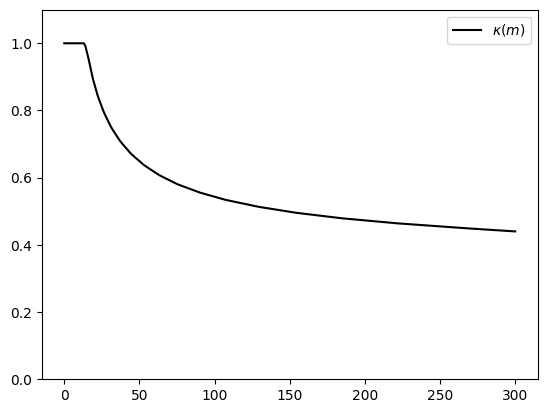
\includegraphics[width=0.6\textwidth]{kFunc_baseline.png}
    \caption{Optimal portfolio share with uncorrelated shocks}
    \label{fig:baseline_portfolio}
\end{figure}

It is obvious that this asymptotic value of $\k$ is increasing in the equity premium. Since the consumer is risk-averse, increasing the volatility of the returns to equity will decrease its attractiveness, thus reducing the optimal value of $\k$ upon an increase in $\s_{\nu}$. The only question, then, is the effect of a positive covariance between income shocks and asset returns on optimal asymptotic portfolio share.

\begin{figure}[h]
    \centering
    \begin{subfigure}{0.49\textwidth}
        \centering
        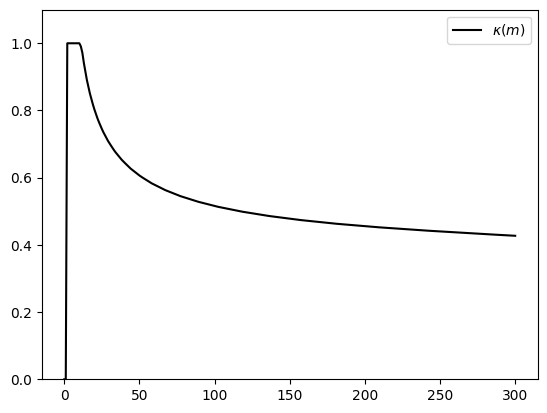
\includegraphics[width=0.8\textwidth]{kFunc_baseline_corrTransFull.png}
        \caption{Transitory shock ($\o_{\nu,\,\z} = 0.014$)}
        \label{subfig:correlated_baseline_transitory}
    \end{subfigure}
    \begin{subfigure}{0.49\textwidth}
        \centering
        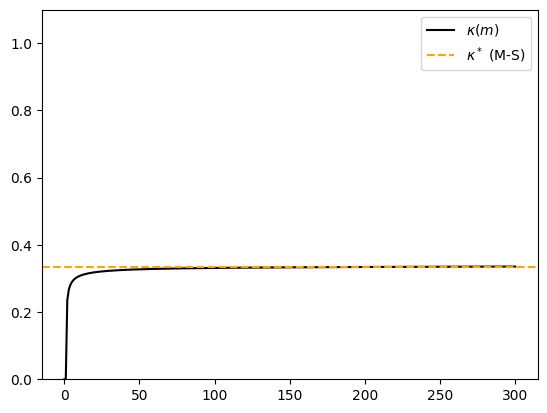
\includegraphics[width=0.8\textwidth]{kFunc_baseline_corr.png}
        \caption{Permanent shock ($\o_{\eta,\,\nu} = 0.008$)}
        \label{subfig:correlated_baseline_permanent}
    \end{subfigure}
    \caption{Optimal portfolio share with a positive correlation between income shocks and asset returns}
    \label{fig:correlated_shock_baseline}
\end{figure}

Figure \ref{fig:correlated_shock_baseline} shows how optimal portfolio share responds to a positive correlation between either of the income shocks and asset returns. Figure \ref{subfig:correlated_baseline_transitory} depicts the case when the transitory shock is correlated with asset returns. Since the optimal portfolio allocation is unaffected for all but the lowest values of $m$ (see section \ref{portfolio_low_wealth}), the asymptotic level of $\k$ remains the same as in the model with uncorrelated shocks. Figure \ref{subfig:correlated_baseline_permanent} shows the portfolio allocation rule under a moderate correlation between permanent income and asset return shocks. Even with a completely different optimal portfolio allocation rule, for high levels of wealth, the optimal portfolio share tends to similar values as in the case with no correlations.

The explanation for this behavior can be found by examining the optimal portfolio share condition, given by:
\[
\E_{t}\bs{(\Rfree_{t+1} - \Rfix)(\Gc_{t+1}c(m_{t+1}))^{-\rho}} = 0
\]
where
\[
m_{t+1} = \frac{\Rc_{t+1}}{\Gc_{t+1}}(m_{t} - c_{t}) + \z_{t+1}
\]
Unquestionably, the covariances between the shocks affect the realized values of $m_{t+1}$, and therefore the realizations of future consumption given by $c(m_{t+1})$. However, for high values of $m_{t}$, given the nature of the consumption function and the low MPC out of current wealth (see section \ref{consumption_baseline}), the variability of the amounts consumed in the future is fairly low. Moreover, consider levels of wealth sufficiently high such that $c(m)$ is large. Naturally, $c_{t+1}^{-\rho}$ is bound to be an extremely small quantity, implying that optimal values of $\k$ are likely to grow increasingly similar under the models with and without correlations in shocks as $m$ grows larger.

\begin{figure}[h]
    \centering
    \begin{subfigure}{0.49\textwidth}
        \centering
        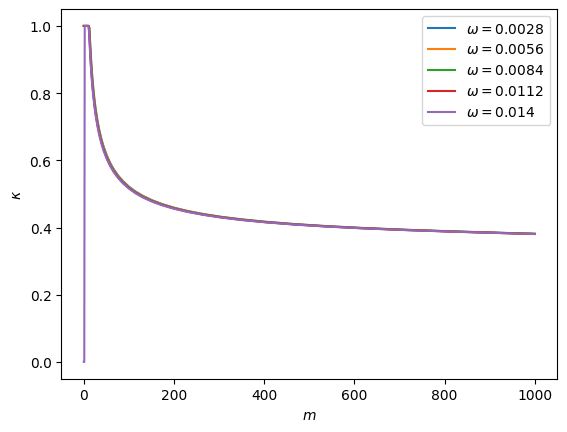
\includegraphics[width=0.8\textwidth]{ShareLimit_transInc_baseline.png}
        \caption{Transitory shock ($\o_{\nu,\,\z} = 0.014$)}
        \label{subfig:shareLimit_baseline_transitory}
    \end{subfigure}
    \begin{subfigure}{0.49\textwidth}
        \centering
        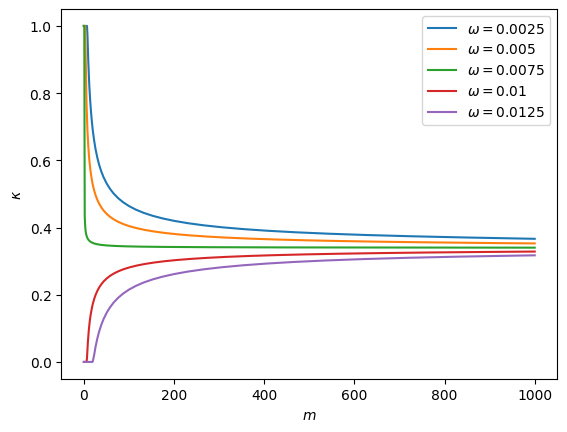
\includegraphics[width=0.8\textwidth]{ShareLimit_permInc_baseline.png}
        \caption{Permanent shock ($\o_{\eta,\,\nu} = 0.008$)}
        \label{subfig:shareLimit_baseline_permanent}
    \end{subfigure}
    \caption{Optimal portfolio share tends to the same value as $m\to \infty$}
    \label{fig:shareLimit_baseline}
\end{figure}

Figure \ref{fig:shareLimit_baseline} provides a rough idea of how the optimal portfolio rule behaves for different levels of correlation between income shocks and asset returns. Figure \ref{subfig:shareLimit_baseline_transitory} shows that correlations between transitory income shocks and asset returns hardly affect the portfolio allocation decision. However, while the portfolio allocation rule is indeed affected significantly by permanent income and asset return shock correlations, as seen in Figure \ref{subfig:shareLimit_baseline_permanent}, the share limit as $m \to \infty$ appears to be unaffected, as the portfolio allocation rules seem to converge. However, given the extremely large savings required to observe such convergence, which is unlikely to be observed of any agent in the model, a change in the correlation between the shocks would indeed affect the distribution of equity holdings. Section \ref{target_wealth} elaborates further on how the equity portfolio share at the target level of wealth is indeed extreme in this model.

\subsubsection{Optimal portfolio share at low wealth}\label{portfolio_low_wealth}

While optimal portfolio shares at large wealth levels are not affected much by the correlation between shocks, we can observe a stark change in the share of the risky asset among individuals whose wealths are less than twice of their permanent incomes.

\begin{figure}[h]
    \centering
    \begin{subfigure}{0.49\textwidth}
        \centering
        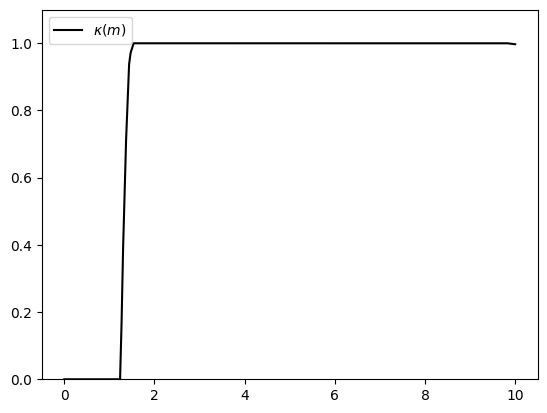
\includegraphics[width=0.8\textwidth]{kFunc_baseline_corrTrans.png}
        \caption{Transitory shock}
        \label{subfig:correlated_poor_transitory}        
    \end{subfigure}
    \begin{subfigure}{0.49\textwidth}
        \centering
        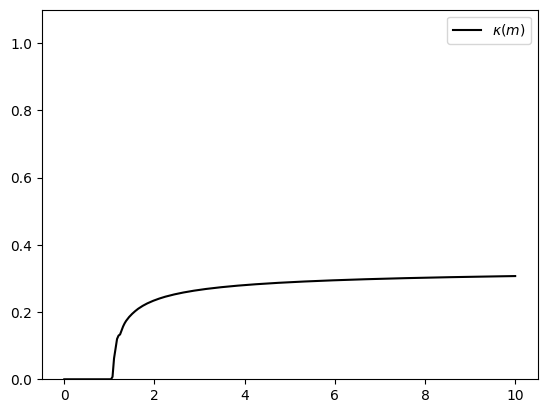
\includegraphics[width=0.8\textwidth]{kFunc_baseline_corrZoomed.png}
        \caption{Permanent shock}
        \label{subfig:correlated_poor_permanent}
    \end{subfigure}
    \caption{Individuals with low wealth invest all their savings in the risk-free asset}
    \label{fig:baseline_correlated_poor}
\end{figure}

Figure \ref{fig:baseline_correlated_poor} shows that agents with normalized wealth less than 2 (somewhere between 1 and 2 to be precise), invest all their savings in the risk-free asset, irrespective of whether asset returns are correlated with transitory or permanent income shocks. At low levels of savings, notice that $\z_{t+1}$ comprises the major component of $m_{t+1}$, and high covariance between $\nu_{t+1}$ and $\z_{t+1}$ implies that low values of $\z_{t+1}$ go with low values of $\nu_{t+1}$. Since the marginal utility of future consumption is high at low values of $m_{t+1}$, which coincides with low values of $\Rfree_{t+1}$, greater weight is placed on instances with low asset returns when taking the expectations in equation (\ref{eq:excess_return}). This lowers the optimal portfolio share of the risky asset, in this case to 0. The other situation is when $\nu$ is correlated with $\eta$. Given the equation of $m_{t+1}$, this actually reduces the variability in $c(m_{t+1})$. However, the positive correlation between $\nu$ and $\eta$ implies that when $\Rfree_{t+1} - \Rfix$ is negative, $\Gc_{t+1}$ is low, implying that $\Gc_{t+1}^{-\rho}$ is higher. Thus, the instances of negative return are weighted higher in the excess return equation. Supposing that $\nu$ and $\eta$ are perfectly correlated, if $\k  1$, then $m_{t+1} - \z_{t+1}$ becomes a constant, and the higher weight accorded to instances with negative return implies that the expectation becomes negative. On the other hand, if $\k = 0$, negative values of $\Rfree_{t+1} - \Rfix$ are coupled with low values of $\Gc_{t+1}$ and therefore higher $m_{t+1}$, implying that the lower marginal utility of normalized consumption under negative excess returns makes $\k = 0$ closer to optimality.

The second aspect is how the optimal portfolio share looks for slightly higher levels of wealth. Upto $m \approx 1.5$, agents consume almost all of their monetary resources and save next to nothing (see section \ref{consumption_baseline}). As such, the high MPC out of consumption causes variability in future monetary resources to translate into variability in future consumption at an almost one-to-one level. After a certain threshold, however, the MPC sharply falls, and the concavity of the consumption function ensures that it continues to fall. Moreover, due to the diminishing marginal utility of consumption and the very low magnitude of the marginal-marginal-utility of consumption, variability in $m_{t+1}$ translates to very little variability in $c(m_{t+1})^{-\rho}$. The analysis of the finite horizon model in section \ref{finite_horizon} highlights the particular relevance of the MPC channel on this effect.

In that light, see that the argument for why optimal $\k$ is low when permanent income shocks and returns are correlated does not crucially depend on the value of $a_{t+1}$ being extremely low, and the optimal $\k$ is always lower than the asymptotic value. However, when looking at the case with correlation between $\z$ and $\nu$, note that the only channel through which there is any effect is the marginal utility of consumption, or $c(m_{t+1})^{-\rho}$. By the discussion above, this has less of an effect at higher values of $m_{t+1}$, and the optimal portfolio allocation rule resembles the one in the model with uncorrelated shocks.

\subsubsection{Optimal consumption policy}\label{consumption_baseline}

While the properties of the consumption function in the buffer stock model are well understood, I reiterate some important features to augment that arguments provided above. Figure \ref{fig:baseline_consumption} shows the optimal consumption function.

\begin{figure}[h]
    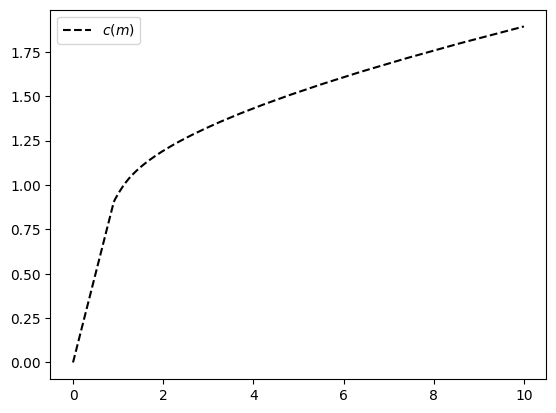
\includegraphics[width=0.6\textwidth]{cFunc_baseline_zoomed.png}
    \caption{Optimal consumption function in the buffer-stock model}
    \label{fig:baseline_consumption}
\end{figure}

Under the artificial no-borrowing constraint, the $c(m) \leq m$, which implies that $c$ is both defined only for $m \geq 0$ and has a kink at the point where the borrowing constraint begins to bind. For this region, the MPC is 1, implying that for low values of $m$, as remarked earlier, the total  savings rate is extremely low. However, the MPC sharply falls beyond this point. The code shows that the optimal consumption policy in the models with correlated shocks remains mostly unchanged. The low MPC for high values of $m$ thus leads to the ineffectiveness of transitory shocks in affecting optimal portfolio choice.

\subsection{Next-to-last period in finite-horizon}\label{finite_horizon}

Due to the convergence properties of the consumption function, we know that the optimal consumption rule in the finite-horizon model for periods sufficiently away from the last period closely approximate the infinite horizon consumption rule. As such, if the next period's consumption is similar to the infinite-horizon consumption, the optimal portfolio allocation rule should also be similar to the infinite-horizon rule. On the other end of this discussion is the period that is next to last.

The consumer in the last period knows that their optimization problem in the last period boils down to maximizing utility from current-period consumption, which implies that $c_T(m_T) = m_T$. The first useful feature of this is that it provides us with a consumption function for which we have an analytical expression, which allows us to rewrite the optimal portfolio allocation condition as:
\[
\E_{T-1}\bs{(\Rfree_{T} - \Rfix)(\Rc_{T}a_{T} + \Gc_{T}\z_{T})^{-\rho}}
\]
First, note that a permanent income growth and transitory income shock are identical in the last period, so to analyze one is to analyze the other. While the coincidence of negative values of $\Rfree_{T} - \Rfix$ and small values of $\Gc_{T}$ still holds true, the MPC out of total monetary resources is a constant 1. As a result, the only channel through which the portfolio choice problem differs at high $m_{T-1}$ as opposed to low is the marginal utility of consumption. Figure \ref{fig:last_prd_portfolio} shows that the optimal portfolio allocation is nearly identical to that in the infinite horizon problem, showing that the effect of correlations between permanent, as opposed to transitory, income shocks and asset returns for moderate values of $m_{T-1}$ is due to the low MPC out of transitory income. However, it also reiterates the point that the low MPC implied by the consumption function in the infinite-horizon problem plays a negligible role in affecting the portfolio choice of the extremely wealthy.

\subsection{Revisiting the excess return equation}

Appendix \ref{excess_return_approx} shows that the excess return equation that determines optimal portfolio allocation can be approximated by
\begin{equation}\label{eq:excess_return_linear}
    \E_{t}\bs{\Rfree_{t+1}} - \Rfix \approx \rho\text{cov}(\D \ln C_{t+1},\,\Rfree_{t+1})
\end{equation}
around steady state values of normalized consumption. Since real consumption change is approximately proportional to permanent income growth around the normalized steady state, a large increase in the covariance between permanent income growth shocks and shocks to $\Rfree_{t+1}$ would then imply that the excess return on equity is less than the covariance between consumption growth and the return on equity, scaled by the relative risk aversion coefficient. One thing to note here is that this approximation depends solely on the covariance, and not the correlation between permanent income growth and the risky rate of return. In fact, for fixed values of expected rates of return and volatility of the risky asset, one can observe that the optimal portfolio allocation rule does not depend much on the volatility of permanent income growth, just its covariance with the risky rate. For instance, under the baseline parameters for equity returns and various levels of permanent income growth volatility, one can observe that poor consumers make the switch from equity to the safe asset at approximately the same level of covariance between logged permanent income growth and equity return shocks.

A second aspect that can be analyzed about the optimal portfolio allocation rule is that for high enough covariance between permanent income growth and asset return shocks, the optimal portfolio share of equity is increasing in wealth, rather than decreasing as before. To understand this, we can look at the version of equation (\ref{eq:excess_return_linear}) that also takes into account the expected consumption growth,
\[
    \E_{t}\bs{\Rfree_{t+1}} - \Rfix \approx (1-\rho\E_{t}\bs{\D\ln C_{t+1}})^{-1}\rho\text{cov}(\D \ln C_{t+1},\,\Rfree_{t+1})
\]
At wealth levels lower than at which the normalized consumption steady state is attained, $\E_{t}\D\ln C_{t+1}$ is large,\footnote{Relative to the average level of permanent income growth} making equity a less desirable asset. On the other hand, for large values of $m_{t}$, as will be elborated on in the next section, agents engage in dissaving behavior (in normalized terms), implying that wealthy agents consume more out of wealth. In such a case, the covariance between consumption growth and equity returns become positive irrespective of the covariance between permanent income growth and equity returns. With $\D\ln C_{t+1}$ decreasing in wealth due to the previously mentioned dissaving behavior, the identical portfolio share limit across the parameterizations of the model can be explained by a convergence in the consumption growth rate as $m \to \infty$ and a decreasing component of permanent income growth in the covariance between consumption growth and equity returns.

\subsection{Behavior around target wealth}\label{target_wealth}

Till now, I have looked at the predictions of the model based on ad-hoc categorizations of poor and wealthy. However, the ability of the model to explain portfolio allocation decisions of individuals also depends on the saving behavior predicted by the model. \citet{Deaton1991} showed that under the satisfaction of a growth impatience condition, individuals save to achieve a target wealth, $m^*$. Assuming that a wealth distribution of agents facing idiosyncratic shocks would be centered around this target level, it would be informative to examine how agents behave at the target.
\begin{figure}[h]
    \centering
    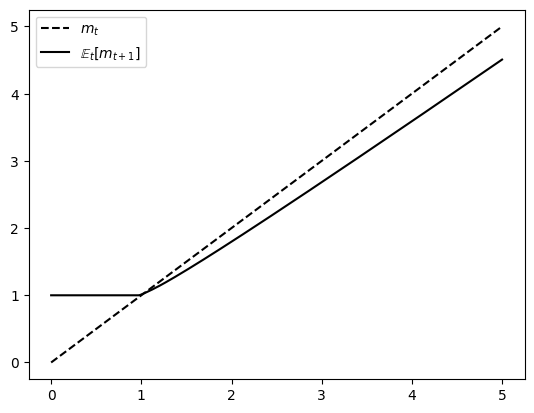
\includegraphics[width=0.6\textwidth]{wealth_transition_baseline.png}
    \caption{Expected next period normalized wealth conditional on current period wealth}
    \label{fig:wealth_transition}
\end{figure}
Figure \ref{fig:wealth_transition} shows how the dynamics of normalized wealth play out from period to period. For low values of $m_{t}$, where savings are zero, next-period wealth is entirely determined by the transitory income shock. Since the expected value of the shock is 1, future wealth is expected to be 1 for all low values of current wealth. Once the no-borrowing constraint stops binding, future wealth is increasing in current wealth. However, it is clear that expected future wealth is lower than current wealth for all values of current wealth slightly greater than 1. In fact, it can be numerically shown that the target level of saving is 2.8 percent of permanent income.

\begin{figure}[h]
    \centering
    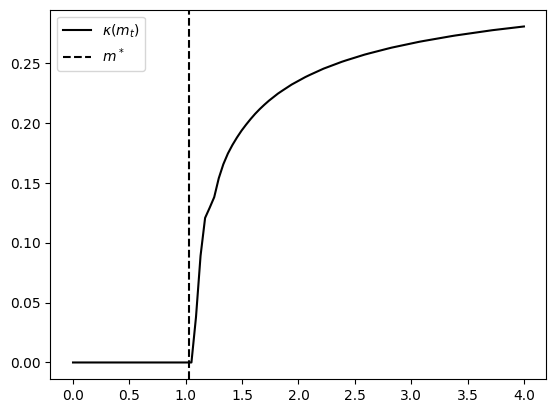
\includegraphics[width=0.6\textwidth]{kFunc_target_baseline.png}
    \caption{Optimal portfolio allocation at the target level of wealth}
    \label{fig:target_wealth_portfolio}
\end{figure}
Figure \ref{fig:target_wealth_portfolio} shows that at the target level of wealth, the optimal portfolio share accorded to equity is actually 0. This is because, under the no-borrowing constraint, the target level of wealth implies very little saving, or $a_{t+1} \approx 0$, where the optimal portfolio share was found to be $0$. If the consumer faces a negative shock to log transitory income, they still have some savings left to allow them to remain at the target level of wealth. When a consumer faces a positive shock to log transitory income, they begin participating in the stock market, and invest a small proportion of their savings in equity. However, from the target wealth, with all savings in the risk-free asset, a consumer's normalized wealth in the next period cannot exceed 1.4 under the current parameterization of the truncated distribution used to model log shocks to income. Then, a large proportion of agents in the wealth distribution should invest no more than 20 percent of their savings in equity, which, of course, would be an extreme prediction. It would, instead, be more intuitive if there was a smoother distribution over equity portfolio share.

A reason for these extreme findings is the binding no-borrowing constraint, and the consumer's heavy dependence on the transitory income for consumption. In fact, if the consumer experiences a negative shock to log transitory income, their consumption would drastically fall, as the target wealth lies just above the kink in the consumption function, and the MPC rises to 1 once the no-borrowing constraint binds. This means that the agent will begin saving once again only after they experience a positive transitory income shock, which prevents them from investing in equity at low levels of savings. In light of this, it can be observed that though the optimal portfolio share quickly rises to 1 in the case of a correlation between asset return and transitory income shocks, the target wealth actually lies below this region, implying that for levels of correlation high enough, the equity share at target wealth drops to 0.

In the next section, I modify the income process and relax the no-borrowing constraint to address this problem.

\appendix
\counterwithin{figure}{section}
\section{Mathematical Appendix}

\subsection{Approximation of expectations}

I recurrently use the following approximation of the expectation of a function of a random variable $X$ around its expectation, $\mu_X$.
\begin{align*}
    f(X) &\approx f(\mu_X) + f'(\mu_X)(X - \mu_X) + \frac{1}{2}f''(\mu_X)(X - \mu_X)^2\\
    \E\bs{f(X)} &\approx f(\mu_X) + \frac{1}{2}f''(\mu_X)\var{X}
\end{align*}
Accordingly, we can compute the expectation of a function of a random vector $X = \bp{X_1,\,...,\,X_k}$ around its expectation vector $\mu_X = \bp{\mu_{X,\,1},\,...,\,\mu_{X,\,k}}$
\begin{align*}
    f(X) &\approx f(\mu_X) + (\nabla f)(\mu_X)\cdot(X - \mu_X) + \frac{1}{2}\tr{H(f)(\mu_X)(X - \mu_X)(X - \mu_X)'}\\
    \E\bs{f(X)} & \approx f(\mu_X) + \frac{1}{2}\tr{H(f)(\mu_X)\S_X}\\
    &= f(\mu_X) + \frac{1}{2}\sum_{i=1}^{k}\sum_{j=1}^{k}\pcd{f(X)}{X_i}{X_j}{\mu_X}\cov{X_i,\,X_j}
\end{align*}
where $\S_X$ is the covariance matrix of $X$, $(\nabla f)(\mu_X)$ is the gradient of $f$, and $H(f)(\mu_X)$ is the Hessian matrix of $f$, both evaluated at $\mu_X$.

\subsection{Approximating the excess return equation}\label{excess_return_approx}

We want to approximate the excess return equation
\[
\E_{t}\bs{(\Rfree_{t+1} - \Rfix)(\Gc_{t+1}c_{t+1})^{-\rho}} = 0
\]
Note that $\Gc_{t+1}c_{t+1} = C_{t+1}$. We can then divide both sides of the equation by $C_{t+1}$ and get
\[
\E_{t}\bs{(\Rfree_{t+1} - \Rfix)\bp{\frac{C_{t+1}}{C_{t}}}^{-\rho}} = 0
\]
The first approximation we can apply is that
\[
\frac{C_{t+1}}{C_{t}} \approx 1 + \D\ln C_{t+1}
\]
for small enough values of $\D\ln C_{t+1}$. Then observe that $(1+x)^{\a} \approx 1 + \a x$ for small $x$. Put together,
\[
\E_{t}\bs{(\Rfree_{t+1} - \Rfix)\bp{1-\rho\D\ln C_{t+1}}} \approx 0
\]
We can then expand this to
\begin{align*}
    \E_{t}\bs{(\Rfree_{t+1} - \Rfix)\bp{1-\rho\D\ln C_{t+1}}} &= \E_{t}\bs{(\Rfree_{t+1} - \Rfix)}\E_{t}\bs{1-\rho\D\ln C_{t+1}} - \text{cov}(\rho\D\ln C_{t+1},\,\Rfree_{t+1})\\
    \E_{t}\bs{\Rfree_{t+1}} - \Rfix &\approx \frac{\rho\text{cov}(\D\ln C_{t+1},\,\Rfree_{t+1})}{1 - \rho\E_{t}\bs{\D\ln C_{t+1}}}
\end{align*}
Around steady state values of normalized consumption, $\E_{t}\D\ln C_{t+1} \approx \E_{t}\D\ln P_{t+1} = \g-\frac{\s_{\eta}^2}{2} \approx 0$, where $\g = \ln \G$. Then
\[
\E_{t}\bs{\Rfree_{t+1}} - \Rfix \approx \rho\text{cov}(\D\ln C_{t+1},\,\Rfree_{t+1})
\]

\subsection{Approximations of covariances}\label{app:covariances}

We want to approximate the covariances of functions of two random variables $X$ and $Y$ around their expectations $\mu_X$ and $\mu_Y$. To do so:
\begin{align*}
    \cov{f(X),\,g(Y)} &= \E\bs{f(X)g(Y)} - \E\bs{f(X)}\E\bs{g(Y)}\\
    \E\bs{f(X)g(Y)} &\approx f(\mu_X)g(\mu_Y) + \frac{1}{2}\bs{f''(\mu_X)g(\mu_Y)\var{X} + f(\mu_X)g''(\mu_Y)\var{Y}} \\&+ f'(\mu_X)g'(\mu_Y)\cov{X,\,Y}\\
    \E\bs{f(X)}\E\bs{g(Y)} &\approx f(\mu_X)g(\mu_Y) + \frac{1}{2}\bs{f''(\mu_X)g(\mu_Y)\var{X} + f(\mu_X)g''(\mu_Y)\var{Y}} \\&+ \frac{1}{4}f''(\mu_X)g''(\mu_Y)\var{X}\var{Y}\\
    \cov{f(X),\,g(Y)} &\approx f'(\mu_X)g'(\mu_Y)\cov{X,\,Y} - \frac{1}{4}f''(\mu_X)g''(\mu_Y)\var{X}\var{Y}
\end{align*}

Using a similar application of the expectations formulae, it can be observed that
\begin{align*}
    \E\bs{f(X_1,\,X_2,\,X_3)g(X_3)} &\approx f(\mu_X)g(\mu_{X,\,3}) + \frac{1}{2}g(\mu_{X,\,3})\sum_{i=1}^{3}\sum_{j=1}^{3}\cov{X_i,\,X_j}\pcd{f(X)}{X_i}{X_j}{\mu_X}\\ &+ g'(\mu_{X,\,3})\sum_{i=1}^{3}\pd{f(X)}{X_i}{\mu_X}\cov{X_i,\,X_3}\\
    &+ \frac{1}{2}g''(\mu_{X,\,3})f(\mu_X)\var{X_3}
\end{align*}
Similarly,
\begin{align*}
    \E\bs{f(X)}\E\bs{g(X_3)} &\approx f(\mu_X)g(\mu_{X,\,3}) + \frac{1}{2}g(\mu_{X,\,3})\sum_{i=1}^{3}\sum_{j=1}^{3}\cov{X_i,\,X_j}\pcd{f(X)}{X_i}{X_j}{\mu_X}\\ &+ \frac{1}{4}g''(\mu_{X,\,3})\var{X_3}\sum_{i=1}^{3}\sum_{j=1}^{3}\pcd{f(X)}{X_i}{X_j}{\mu_X}\\
    &+ \frac{1}{2}f(\mu_X)\var{X_3}g''(\mu_{X,\,3})
\end{align*}
Then
\begin{align*}
    \cov{f(X),\,g(X_3)} &\approx g'(\mu_{X,\,3})\sum_{i=1}^{3}\pd{f(X)}{X_i}{\mu_X}\cov{X_i,\,X_3}\\ &- \frac{1}{4}g''(\mu_{X,\,3})\var{X_3}\sum_{i=1}^{3}\sum_{j=1}^{3}\pcd{f(X)}{X_i}{X_j}{\mu_X}
\end{align*}

\subsection{Approximation of covariance of consumption and equity returns}\label{app:cons_return_cov}

We want to approximate the expression
\[
\cov{\D\ln C_{t+1},\,\Rfree_{t+1}}
\]
which features in the approximate excess return equation. We can start by noting that $C_t$ is a known quantity, so $\cov{\D\ln C_{t+1},\,\Rfree_{t+1}} = \cov{\ln C_{t+1},\,\Rfree_{t+1}}$. Thereafter
\begin{align*}
    C_{t+1} &= \G\psi_{t+1}P_tc_{t+1}\\
    \ln C_{t+1} &= \ln \G + \ln P_t + \ln \psi_{t+1}+ \ln c_{t+1}\\
    \cov{\ln C_{t+1},\,\Rfree_{t+1}} &= \Rfree\bs{\cov{\ln \psi_{t+1},\,\nu_{t+1}} + \cov{\ln c_{t+1},\,\nu_{t+1}}}
\end{align*}
Note that $\E\bs{\ln \psi_{t+1}} = -\frac{\s_{\psi}^2}{2}$ and $\E\bs{\ln \nu_{t+1}} = -\frac{\s_{\nu}^2}{2}$. We can then approximate
\begin{align*}
    \cov{\ln \psi_{t+1},\,\nu_{t+1}} &= \cov{\ln \psi_{t+1},\,\exp(\ln \nu_{t+1})}\\
    &\approx \exp\bp{-\frac{\s_{\nu}^2}{2}}\cov{\ln \psi_{t+1},\,\ln \nu_{t+1}}\\
    &\approx \bp{1 - \frac{\s_{\nu}^2}{2}}\o_{\psi,\,\nu}\\
    &\approx \o_{\psi,\,\nu}
\end{align*}
Now observe that with $m_t$ known and $c_t = c(m_t)$ subsequently determined, $c_{t+1}$ can be written as $\hat{c}(\psi_{t+1},\,\t_{t+1},\,\nu_{t+1})$, where
\[
\hat{c}(\psi_{t+1},\,\t_{t+1},\,\nu_{t+1}) \equiv c\bp{\frac{\Rfix + \vs(\Rfree\nu_{t+1} - \Rfix)}{\G\psi_{t+1}}\bp{m_t - c_t} + \t_{t+1}}
\]
Define $\bar{m}$ as
\[
\bar{m} = \frac{\Rfix + \vs(\Rfree - \Rfix)}{\G}\bp{m_t - c_t} + 1
\]
Then, setting $f \equiv \ln \circ \hat{c}$ and $g$ as the identity function, we can approximate
\begin{align*}
    \cov{\ln \circ \hat{c}(\psi_{t+1},\,\t_{t+1},\,\nu_{t+1}),\,\nu_{t+1}} & \approx \var{\nu_{t+1}} \frac{c'(\bar{m})}{c(\bar{m})}\frac{\vs\Rfree}{\G}(m_t - c_t)\\
    &- \cov{\psi_{t+1},\,\nu_{t+1}}\frac{c'(\bar{m})}{c(\bar{m})}\frac{\Rfix + \vs(\Rfree - \Rfix)}{\G}(m_t - c_t)\\
    &+ \cov{\t_{t+1},\,\nu_{t+1}}\frac{c'(\bar{m})}{c(\bar{m})}
\end{align*}
Now we can see that
\begin{align*}
    \cov{e^X,\,e^Y} &\approx \exp\bp{-\frac{\s_X^2 + \s_Y^2}{2}}\cov{X,\,Y} - \frac{1}{4}{\s_X^2\s_Y^2}\exp\bp{-\frac{\s_X^2 + \s_Y^2}{2}}\\
    &\approx \cov{X,\,Y} \tag{for small $\s_X$ and $\s_Y$}
\end{align*}
For the NBC model, $\t_{t+1} = \z_{t+1}$, so $\cov{\t_{t+1},\,\nu_{t+1}} \approx \o_{\z,\,\nu}$. However, even in the NIR model, note that $\E\bs{\t_{t+1}}$ and $\E\bs{\nu_{t+1}}$ are unchanged, while
\[
\E\bs{\t_{t+1}\nu_{t+1}} = \wp\cdot 0 + (1-\wp)\frac{\E\bs{\z_{t+1}\nu_{t+1}}}{1-\wp} = \E\bs{\z_{t+1}\nu_{t+1}}
\]
Thus,
\begin{align*}
    \cov{\D\ln C_{t+1},\,\Rfree_{t+1}} &\approx \Rfree\bp{\o_{\psi,\,\nu} + \frac{c'(\bar{m})}{c(\bar{m})}\bp{(m_t - c_t)\bp{\frac{\vs\Rfree\s_{\nu}^2 - (\Rfix + \vs(\Rfree - \Rfix))\o_{\psi,\,\nu}}{\G}} + \o_{\z,\,\nu}}}
\end{align*}

\subsection{Proof of Proposition \ref{prop:low_wealth_share}}\label{pf:low_wealth_share}

Note from Appendix \ref{app:cons_return_cov}, that
\begin{align*}
    \rho\cov{\ln \D C_{t+1},\,\Rfree_{t+1}} &\approx \rho\Rfree\bp{\o_{\psi,\,\nu} + \frac{c'(\bar{m})}{c(\bar{m})}\bp{(m_t - c_t)\bp{\frac{\vs\Rfree\s_{\nu}^2 - (\Rfix + \vs(\Rfree - \Rfix))\o_{\psi,\,\nu}}{\G}} + \o_{\z,\,\nu}}}
\end{align*}
By Lemma \ref{lm:nbc_kink}, there exists $\tilde{m} > 0$ such that $c(m) = m$ for $m \leq \tilde{m}$. For such $m$,
\begin{align*}
    \rho\cov{\ln \D C_{t+1},\,\Rfree_{t+1}} &\approx \rho\Rfree\bp{\o_{\psi,\,\nu} + \frac{c'(1)}{c(1)}\o_{\z,\,\nu}}
\end{align*}
as $a_{t+1} = 0$ and $\bar{m} = \E\bs{\t_{t+1}} = 1$. Since $\rho\cov{\D\ln C_{t+1},\,\Rfree_{t+1}}$ is continuous in $m$,\footnote{\citet{Carroll2024b} show that $c$ is twice continuously differentiable in $m$.} if $\rho\cov{\ln \D C_{t+1},\,\Rfree_{t+1}} > \Rfree - \Rfix$ for $m < \tilde{m}$, it is also  true for $m < \tilde{m} + \e$, for $\e > 0$ and any $\vs \in \bs{0,\,1}$. Thus, under the conditions for optimality, $\vs(m) = 0$ for all such $m$. Likewise, $\vs(m) = 1$ for $m < \tilde{m} + \e$ if $\rho\cov{\ln \D C_{t+1},\,\Rfree_{t+1}} < \Rfree - \Rfix$ for $m' < \tilde{m}$. Defining $m^*$ as the supremum of such $m$, we have the binary policy rule, as in the result. The only thing left to prove is that $\tilde{\o} = \frac{\Rfree - \Rfix}{\rho\Rfree}$. That is obvious upon dividing both sides of the excess return equation by $\rho\Rfree$.

\subsection{Proof of Proposition \ref{prop:wealth_share_diff}}\label{pf:wealth_share_diff}

% Note from Appendix \ref{app:cons_return_cov}, we can rewrite the excess return equation as
% \begin{align*}
%     \Rfree - \Rfix &\approx \rho\Rfree\bp{\o_{\psi,\,\nu} + \frac{c'(\bar{m})}{c(\bar{m})}\bp{(m_t - c_t)\bp{\frac{\vs\Rfree\s_{\nu}^2 - (\Rfix + \vs(\Rfree - \Rfix))\o_{\psi,\,\nu}}{\G}} + \o_{\z,\,\nu}}}\\
%     \vs(m) &\approx \frac{\G}{\Rfree\s_{\nu}^2 - (\Rfree - \Rfix)\o_{\psi,\,\nu}}\bp{\frac{c(\bar{m})}{c'(\bar{m})\bp{m - c(m)}}\bp{\frac{\Rfree - \Rfix}{\rho\Rfree} - \o_{\psi,\,\nu}} + \frac{\o_{\z,\,\nu}}{m - c(m)} - \frac{\Rfix\o_{\psi,\,\nu}}{\G}}
% \end{align*}
% After the kink in the consumption function, the optimal portfolio share is differentiable in wealth, as the consumption function is twice-continuously differentiable in wealth. First, note
% \[
% \frac{d}{dm}\frac{c(\bar{m})}{c'(\bar{m})\bp{m - c(m)}} = \frac{c'(\bar{m})^2\b[]}
% \]


% The derivative of the optimal portfolio share is then
% \[
% \vs'(m) \approx \frac{\G}{\Rfree\s_{\nu}^2 - (\Rfree - \Rfix)\o_{\psi,\,\nu}}\bp{}
% \]


Note from Appendix \ref{app:cons_return_cov}, the excess return equation is approximated as
\begin{align*}
    \Rfree - \Rfix &\approx \rho\Rfree\bp{\o_{\psi,\,\nu} + \frac{c'(\bar{m})}{c(\bar{m})}\bp{(m_t - c_t)\bp{\frac{\vs\Rfree\s_{\nu}^2 - (\Rfix + \vs(\Rfree - \Rfix))\o_{\psi,\,\nu}}{\G}} + \o_{\z,\,\nu}}}
\end{align*}
Note,
\[
\bar{m}'(m) = \frac{\Rfix + \vs(\Rfree - \Rfix)}{\G} > 0
\]
and
\[
\frac{d}{dm}\frac{c'(\bar{m})(m - c(m))}{c(\bar{m})} = \frac{c(\bar{m})(c''(\bar{m})(m - c(m))\bar{m}'(m) + c'(\bar{m})(1 - c'(m))) - c'(\bar{m})^2(m - c(m))\bar{m}'(m)}{c(\bar{m})^2}
\]
By the concavity of $c$, the above derivative is negative. Supposing that $\o_{\z,\,\nu} = 0$,\footnote{This covariance becomes inconsequential with wealth, as $\frac{c'(\bar{m})}{c(\bar{m})}$ sharply falls} we only care about the positivity or negativity of the term
\[
    \vs\Rfree\s_{\nu}^2 - (\Rfix + \vs(\Rfree - \Rfix))\o_{\psi,\,\nu}
\]
This term is positive if and only if
\begin{align*}
    \o_{\psi,\,\nu} &< \frac{\vs\Rfree\s_{\nu}^2}{\Rfix + \vs(\Rfree - \Rfix)}\\
    &\leq \s_{\nu}^2
\end{align*}
Therefore, if $\o_{\psi,\,\nu} \geq \s_{\nu}^2$, this term is non-positive, and $\cov(\ln \D C_{t+1},\,\Rfree_{t+1})$ is increasing in wealth. As such, the optimal portfolio share is decreasing in wealth. On the other hand, if $\o_{\psi,\,\nu} < \s_{\nu}^2$, the term is positive when $\vs = 1$, and negative when $\vs = 0$. Thus, there exists a threshold $\vs$ such that the optimal portfolio share is increasing in wealth below this portfolio share. This threshold is given by
\[
\vs < \frac{\Rfix\o_{\psi,\,\nu}}{\Rfree\s_{\nu}^2 - (\Rfree - \Rfix)\o_{\psi,\,\nu}}
\]
Now, suppose $\o_{\psi,\,\nu} = \tilde{\o} = \frac{\Rfree - \Rfix}{\rho\Rfree}$. Then
\begin{align*}
    \frac{\Rfix\frac{\Rfree - \Rfix}{\rho\Rfree}}{\Rfree\s_{\nu}^2 - \frac{(\Rfree - \Rfix)^2}{\rho\Rfree}} &= \frac{\Rfix(\Rfree - \Rfix)}{\rho\Rfree^2\s_{\nu}^2 - (\Rfree - \Rfix)^2}
\end{align*}
Since the threshold value is increasing in $\o_{\psi,\,\nu}$, the optimal portfolio share is increasing in wealth for $\o_{\psi,\,\nu} > \tilde{\o}$ as long it is below this share share. Likewise, the optimal portfolio share is decreasing in wealth for $\o_{\psi,\,\nu} < \tilde{\o}$ as long as it is above this share. As such, we must only show that in each case, the optimal portfolio share lies on either side of this threshold.

Rearranging the excess return equation, the optimal portfolio rule can be written as
\[
    \vs(m) \approx \frac{\G}{\Rfree\s_{\nu}^2 - (\Rfree - \Rfix)\o_{\psi,\,\nu}}\bp{\frac{c(\bar{m})}{c'(\bar{m})\bp{m - c(m)}}\bp{\frac{\Rfree - \Rfix}{\rho\Rfree} - \o_{\psi,\,\nu}} - \frac{\Rfix\o_{\psi,\,\nu}}{\G}}
\]
First, note that differentiating the right hand side w.r.t $\o_{\psi,\,\nu}$ reveals that it is decreasing in $\o_{\psi,\,\nu}$. Thus, the optimal portfolio share is decreasing in $\o_{\psi,\,\nu}$. Now, note that the right hand side is decreasing in $\o_{\psi,\,\nu},$\footnote{Also see that $\cov{\ln C_{t+1},\,\Rfree_{t+1}}$ is increasing in $\o_{\psi,\,\nu}$, so $\vs$ is decreasing in $\o_{\psi,\,\nu}$.} so $\vs$ is decreasing in $\o_{\psi,\,\nu}$. Note, then, for $\o_{\psi,\,\nu} = \tilde{\o}$,
\begin{align*}
    \vs(m) &\approx \frac{\Rfix(\Rfree - \Rfix)}{\rho\Rfree^2\s_{\nu}^2 - (\Rfree - \Rfix)^2}
\end{align*}
Therefore, $\vs(m)$ is greater than the threshold share if $\o_{\psi,\,\nu} < \tilde{\o}$, and lower otherwise. As such, $\vs(m)$ is increasing in wealth for $\o_{\psi,\,\nu} > \tilde{\o}$, and decreasing otherwise. Note that for plausible values of $\Rfree$, $\Rfix$, and $\s_{\nu}$, $(\Rfree^2 - 1)\rho\s_{\nu}^2 - (\Rfree - \Rfix)^2 \approx 0$ and $\Rfix \approx 1$. Thus, the threshold value of $\vs$ is approximately
\begin{align*}
    \vs(m) &= \frac{\Rfix(\Rfree - \Rfix)}{\rho\Rfree^2\s_{\nu}^2 - (\Rfree - \Rfix)^2}\\
    &= \frac{\Rfix(\Rfree - \Rfix)}{\rho\s_{\nu}^2 + (\Rfree^2 - 1)\rho\s_{\nu}^2 - (\Rfree - \Rfix)^2}\\
    &\approx \frac{\Rfree - \Rfix}{\rho\s_{\nu}^2}
\end{align*}
Note that this is the Merton-Samuelson share.


\subsection{Proof of Proposition \ref{prop:high_wealth_share}}\label{pf:high_wealth_share}

Note from Appendix \ref{app:cons_return_cov}, that
\begin{align*}
    \rho\cov{\ln \D C_{t+1},\,\Rfree_{t+1}} &\approx \rho\Rfree\bp{\o_{\psi,\,\nu} + \frac{c'(\bar{m})}{c(\bar{m})}\bp{(m_t - c_t)\bp{\frac{\vs\Rfree\s_{\nu}^2 - (\Rfix + \vs(\Rfree - \Rfix))\o_{\psi,\,\nu}}{\G}} + \o_{\z,\,\nu}}}
\end{align*}
Since the right hand side is differentiable in $m$, we can determine the approximate limit of the optimal portfolio share from the limit of the right hand side as $m$ approaches infinity. \citet{Carroll2024b} show that $c'(m) \to \underline{\k} \geq 0$ as $m \to \infty$, where $\underline{\k} > 0$ subject to the satisfaction of a growth impatience condition. Thus,
\begin{align*}
    \lim_{m\to\infty}\frac{c'(\bar{m})(m - c(m))}{c(\bar{m})} &= \lim_{m\to\infty}\frac{c'(\bar{m})\frac{m-c(m)}{m}}{\frac{c(\bar{m})}{m}}\\
    \lim_{m\to\infty}\frac{m - c(m)}{m} &= \lim_{m\to\infty}1 - c'(m)\\
    &= 1 - \underline{\k}\\
    \lim_{m\to\infty}\frac{c(\bar{m})}{m} &= \lim_{m\to\infty}c'(\bar{m})\bar{m}'(m)\\
    \implies \lim_{m\to\infty}\frac{c'(\bar{m})(m - c(m))}{c(\bar{m})} &= \lim_{m\to\infty}\frac{c'(\bar{m})(1-c'(\bar{m}))}{c'(\bar{m})\bar{m}'(m)}\\
    &= \lim_{m\to\infty}\frac{(1-c'(\bar{m}))}{\bar{m}'(m)}\\
    &= \frac{\G}{\Rfix + \vs(\Rfree - \Rfix)}
\end{align*}
Note that $\lim_{m\to\infty}\frac{c'(\bar{m})}{c(\bar{m})} = 0$, so the limit of the covariance term is
\[
    \lim_{m\to\infty}\rho\cov{\ln \D C_{t+1},\,\Rfree_{t+1}} \approx \rho\Rfree\frac{\vs\Rfree\s_{\nu}^2}{\Rfix + \vs(\Rfree - \Rfix)}
\]
Substituting this back into the excess return equation,
\begin{align*}
    \Rfree - \Rfix \approx \frac{\rho\Rfree^2\s_{\nu}^2\vs}{\Rfix + \vs(\Rfree - \Rfix)}\\
    \Rfix(\Rfree - \Rfix) + \vs(\Rfree - \Rfix)^2 \approx \rho\Rfree^2\s_{\nu}^2\vs\\
    \lim_{m\to\infty}\vs \approx \frac{\Rfix(\Rfree - \Rfix)}{\rho\Rfree^2\s_{\nu}^2 - (\Rfree - \Rfix)^2}
\end{align*}
Thus, it is evident that the optimal portfolio share is independent of the covariance between income and returns on equity as wealth grows arbitrarily large. By the approximation employed in the proof of Proposition \ref{prop:wealth_share_diff}, this limit is approximately the Merton-Samuelson share. That is
\[
\lim_{m\to\infty}\vs \approx \frac{\Rfree - \Rfix}{\rho\s_{\nu}^2}
\]

\section{Computational Appendix}

\subsection{Solving the model}\label{app:seq_egm}

I solve the model using a sequential application of the endogenous grid method \citep{Carroll2006}, dividing a period into two subperiods, the first stage involving a consumption decision ($c$), and the second involving the portfolio optimization problem ($\vs$). This description largely pertains to the finite-horizon version, though the infinite-horizon solution merely replaces periods with a sequence of guesses.

Construct a grid of assets $\Ac = \bs{\underline{a} = a_1 < a_2 < ... < a_k = \overline{a}}$. To solve the problem pertaining to any period $t$, observe from equation (\ref{eq:excess_return}) that whenever $a_i \neq 0$, the optimal share of risky assets is given by the choice of $\hat{\vs}_{t+1}(a_i) \in [0,\,1]$ such that
\begin{equation}\label{eq:kappa}
n^{-3}\G_{t+1}^{-\rho}\sum_{j=1}^{n^3}(\Rfree\nu_i - \Rfix)(\psi_{j}c_{t+1}(m_{ij}))^{-\rho} = 0
\end{equation}
where
\[
m_{ij} = \frac{\Rfix + \hat{\vs}_{t+1}(a_i)(\Rfree\nu_j - \Rfix)}{\G_{t+1}\psi_{j}}a_i + \t_j
\]
The problem then becomes a root-finding operation pertaining to a function of $\hat{\vs}$, which, given a policy function $c_{t+1}$, yields an optimal level of $\hat{\vs}$ for each $a_i$. Denote this pair as $(a,\,\hat{\vs})_{i}$, and the resulting effective return $\Rfix + \hat{\vs}_{i}(\Rfree\nu_{j} - \Rfix)$ for each value of the shocks as $\Rc_{ij}$.

For each \textit{end-of-period} outcome $(a,\,\hat{\vs})_i$, given $c_{t+1}$, we can use the consumption Euler equation to get
\[
[\hat{c}_t(a_i,\,\hat{\vs}_i)]^{-\rho} = \b\G_{t+1}^{-\rho} n^{-3}\sum_{j=1}^{n^3}\Rc_{ij}(\psi_{j}c_{t+1}(m_{ij}))^{-\rho}
\]
where $\hat{c}$ denotes that this yields a consumed function of the assets and portfolio share.
This function is then given by
\[
\hat{c}_{t}(a_i,\,\hat{\vs}_i) = \bs{\b\G_{t+1}^{-\rho}n^{-3}\sum_{j=1}^{n^3}\Rc_{ij}(\psi_{j}c_{t+1}(m_{ij}))^{-\rho}}^{-\frac{1}{\rho}}
\]
Now we have a vector of $\hat{c}_i$ corresponding to each $(a,\,\hat{\vs})_i$. Since $m_{t} = c_{t} + a_{t+1}$, we can construct the grid $\Mc$ with each $m_i \in \Mc$ given by $m_i = \hat{c}_i + a_i$, where $\hat{c}_{i} = \hat{c}_{t}(a_i,\,\hat{\vs}_i)$. We can now rewrite $c_t(m_i) = \hat{c}_t(a_i,\,\hat{\vs}_i)$ and $\vs_{t+1}(m_i) = \hat{\vs}_{t+1}(a_i)$, and interpolate to get the policy functions $(c_{t}(m),\,\vs_{t+1}(m)) = g_{t}(m)$ for period $t$.\footnote{While I use linear interpolation by default, cubic-spline interpolation yields similar results for the consumption function. However, due to drastic directional changes in the optimal portfolio share, spline interpolation sometimes suggests a portfolio share outside the interval $[0,\,1]$.} In the finite-horizon case, the model can be solved using $c_{T}(m) = m$ as the initial policy function and iterating backwards till period 0. For the infinite-horizon case, I use a guess $c_{0}(m)$ to obtain a sequence of guesses $\bc{c_{k}(m),\,\vs_{k}(m)}_{k=0}^{K}$ that converge to the true policy functions $c(m)$ and $\vs(m)$. Since my focus is not on life-cycle applications, I solve each model with a constant permanent growth factor $\G$.

\subsection{Baseline consumption}\label{consumption_baseline}

\begin{figure}[H]
    \centering
    \includegraphics[width=0.6\textwidth]{\NBCConsumption}
    \caption{Optimal consumption function in the buffer-stock model}
    \label{fig:baseline_consumption}
\end{figure}

\subsection{Last Period Optimal Portfolio Allocation}

\begin{figure}[h]
    \centering
    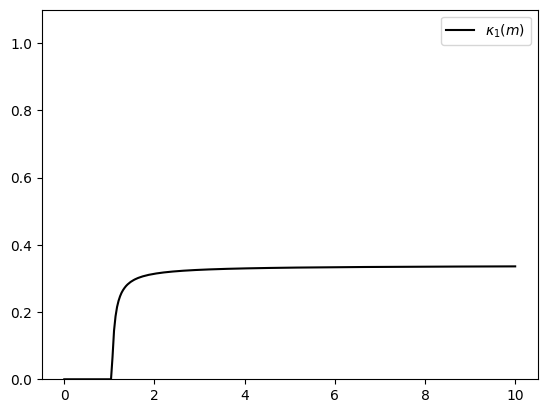
\includegraphics[width=0.6\textwidth]{kFunc_LastPrd.png}
    \caption{Optimal portfolio allocation in the second-to-last period}
    \label{fig:last_prd_portfolio}
\end{figure}

\printbibliography

% \printbibliography

\bibliographystyle{agsm}
\bibliography{correlated_shocks_equity_premium}

\end{document}